\documentclass[12pt,a4paper]{article}
\usepackage[utf8]{inputenc}
\usepackage[utf8]{vietnam}
\usepackage{amsmath,amsfonts,amssymb}
\usepackage[margin=0.9in]{geometry}
\usepackage{graphicx}
\graphicspath{ {images/} }
\usepackage{wrapfig}

\usepackage{subfig}
\usepackage{indentfirst}
\usepackage{xcolor}
\usepackage{color}
\usepackage{booktabs}
\usepackage{diagbox}
\usepackage{multicol}
\usepackage{multirow}
\usepackage[unicode,hidelinks=true]{hyperref}	% Tạo các siêu liên kết
\hypersetup{pdftitle={Đánh số cho các phần, các chương và các mục trong tài liệu LaTeX},
	pdfauthor={Thi Minh Nhựt},
	pdfsubject={LaTeX Tutorials},
	pdfkeywords={latex, article, report, book, part, chapter, section, subsection, subsubsection, subsubsubsection, paragraph, subparagraph},
	bookmarks=true,
	bookmarksopen=true
}

\usepackage{fancyvrb}
\usepackage{verbatim}

\usepackage[labelfont={bf}]{caption}
\captionsetup[figure]{name=Ví dụ}


\setcounter{tocdepth}{5}
\setcounter{secnumdepth}{5}
% Định nghĩa lệnh parasection từ lệnh paragraph
\newcommand{\parasection}[1]{\paragraph{#1}\mbox{}\medskip\par}

% Định nghĩa lệnh subparasection từ lệnh subparagraph
\newcommand{\subparasection}[1]{{\setlength{\parindent}{0pt}\subparagraph{#1}\mbox{}\medskip \par}}


\newcommand{\tab}[1]{\textbf{Bảng~#1}}
\newcommand{\ex}[1]{\textbf{Ví dụ~#1}}
\newcommand{\head}[1]{\textbf{#1}}
\newcommand{\command}[1]{\texttt{\string#1}}

\title{\bfseries \huge Đánh số cho các phần, các chương và các mục trong tài liệu \LaTeX}
\author{\Large Thi Minh Nhựt \bigskip \\  \Large \texttt{thiminhnhut@gmail.com}}
\date{\Large Ngày 06 tháng 02 năm 2017}
\begin{document}
\maketitle
\tableofcontents

\begin{thebibliography}{99}
	\bibitem{section-math2it} \href{http://math2it.com/}{\textbf{Math2IT}}, \href{https://goo.gl/HuiPpu}{\textit{Tùy chỉnh cách đánh số chapter, section, subsection trong \LaTeX}}, \href{http://math2it.com/category/latex/}{Chủ đề \LaTeX}.
	
	\bibitem{counters-sharelatex} \href{https://www.sharelatex.com}{\textbf{Share LaTeX}}, \href{https://goo.gl/weJlVt}{\emph{Counters}}, \href{https://www.sharelatex.com/learn}{Help Documents}.
	
	\bibitem{section-sharelatex} \href{https://www.sharelatex.com}{\textbf{Share LaTeX}}, \href{https://goo.gl/e5ncGK}{\emph{Sections and chapters}}, \href{https://www.sharelatex.com/learn}{Help Documents}.   
\end{thebibliography}

\newpage
\section{Giới thiệu}
	Một trong những tính năng của \LaTeX\ là khả năng đánh số các phần, các chương và các mục trong tài liệu một cách tự động và khoa học. \LaTeX\ cung cấp cho chúng ta 7 cấp độ đánh số, tùy thuộc vào loại tài liệu mà có những cấp độ phù hợp được trình bày trong \tab{\ref{Tab:7cap-danhso}}.\\		
	
	Phần hướng dẫn bên dưới đã được thử nghiệm thành công với phiên bản \TeX Live 2015 được cài đặt trên hệ điều hành Ubuntu 16.04 và sử dụng trình soạn thảo \TeX Maker để biên dịch với PDF \LaTeX. \\
	
	File \TeX\ của bài hướng dẫn được lưu ở địa chỉ \url{https://github.com/thiminhnhut/latex/tree/master/tips/danhso-cacmuc-tronglatex}, chúng ta có thể dùng file này để làm mẫu thực hiện soạn theo.\\
	
	Lệnh \Verb|\part| áp dụng cho lớp \Verb|book|, lệnh \Verb|\chapter| áp dụng cho lớp \Verb|report| và lớp \Verb|book|. Các lệnh còn lại có đủ trong cả ba lớp \Verb|article|, lớp \Verb|report| và lớp \Verb|book|.

	\begin{table}[h]
		\begin{center}
			\begin{tabular}{cllll}\toprule
				\head{Cấp độ} & \head{Lệnh}  & \multicolumn{3}{c}{\head{Cách đánh số trong các lớp}} \\ \midrule
				&  & \Verb|article| & \Verb|report| & \Verb|book| \\ \midrule
				-1  & \Verb|\part{Tên phần}| & &  & \textbf{I} \\ \midrule
				0  & \Verb|\chapter{Tên chương}| & & \textbf{1} & \textbf{1} \\ \midrule
				1  & \Verb|\section{Tên section}| & \textbf{1} & \textbf{1.1} & \textbf{1.1} \\ \midrule
				2  & \Verb|\subsection{Tên subsection}| & \textbf{1.1} & \textbf{1.1.1} & \textbf{1.1.1} \\ \midrule
				3  & \Verb|\subsubsection{Tên subsubsection}| & \textbf{1.1.1} &  &  \\ \midrule
				4  & \Verb|\paragraph{Nội dung}| &  &  &  \\ \midrule
				5  & \Verb|\subparagraph{Nội dung}| &  &  &  \\ \bottomrule
			\end{tabular}
		\end{center}
		\caption{Các cấp độ đánh số và cách đánh số mặc định với các lớp trong \LaTeX} \label{Tab:7cap-danhso}
	\end{table}		
	
\section{Hiện số cho những cấp độ bị ẩn bởi mặc định trong các lớp của \LaTeX}
	Theo phần trình bày trong \tab{\ref{Tab:7cap-danhso}}, trong mỗi lớp có một số cấp độ đánh số bị ẩn bởi mặc định và các cấp độ bị ẩn thì nội dung của chúng cũng không được tự động thêm vào mục lục.\\ 
	
	Phần hướng dẫn bên dưới, chúng ta sẽ tìm hiểu cách để hiển thị số của các cấp độ bị ẩn và thêm nội dung của chúng vào mục lục.

\subsection{Đánh số và thêm nội dung của các cấp độ vào mục lục}
	\begin{itemize}
		\item Sử dụng các lệnh bên dưới (đặt trước \Verb|\begin{document}|), với \Verb|n| là các cấp độ được cho trong \tab{\ref{Tab:7cap-danhso}}.
			\begin{itemize}
				\item Đánh số đến cấp độ thứ \Verb|n|: \Verb|\setcounter{secnumdepth}{n}|

				\item Thêm nội dung của những cấp độ đến cấp độ thứ \Verb|n| vào mục lục (khi sử dụng lệnh \Verb|\tableofcontents|): \Verb|\setcounter{tocdepth}{n}|
			\end{itemize}

		\item Ví dụ, cách đánh số cho các cấp độ bị ẩn trong \tab{\ref{Tab:7cap-danhso}} được trình bày trong \tab{\ref{Tab:capdo-bian}}.				
			\begin{table}[h]
				\begin{center}
					\begin{tabular}{lllll}\toprule
						\multirow{2}{*}{\head{Lệnh}} & \multirow{2}{4.6cm}{\head{Lệnh đánh số và thêm nội dung vào mục lục}} & \multicolumn{3}{c}{\head{Cách đánh số trong các lớp}} \\ \cmidrule{3-5}
						& & \Verb|article| & \Verb|report| & \Verb|book| \\ \midrule
						\multirow{3}{*}{\command{\subsubsection}} & \Verb|\setcounter{secnumdepth}{3}| &  & \multirow{3}{*}{\textbf{1.1.1.1}} & \multirow{3}{*}{\textbf{1.1.1.1}} \\ 
						& \Verb|\setcounter{tocdepth}{3}| &  &  &  \\
						& Là mặc định trong lớp \Verb|article| &  &  &  \\ \midrule
						\multirow{2}{*}{\command{\paragraph}} & \Verb|\setcounter{secnumdepth}{4}| & \multirow{2}{*}{\textbf{1.1.1.1}} & \multirow{2}{*}{\textbf{1.1.1.1.1}} & \multirow{2}{*}{\textbf{1.1.1.1.1}} \\ 
						& \Verb|\setcounter{tocdepth}{4}| &  &  &  \\ \midrule						
						\multirow{2}{*}{\command{\subparagraph}} & \Verb|\setcounter{secnumdepth}{5}| & \multirow{2}{*}{\textbf{1.1.1.1.1}} & \multirow{2}{*}{\textbf{1.1.1.1.1.1}} & \multirow{2}{*}{\textbf{1.1.1.1.1.1}} \\ 
						& \Verb|\setcounter{tocdepth}{5}| &  &  &  \\ \bottomrule
					\end{tabular}
				\end{center}
				\caption{Đánh số các cấp độ bị ẩn trên \tab{\ref{Tab:7cap-danhso}} và thêm nội dung của chúng vào mục lục} \label{Tab:capdo-bian}
			\end{table}				

		\item Khi sử dụng lệnh \Verb|\setcounter{secnumdepth}{5}| và \Verb|\setcounter{tocdepth}{5}|, chúng ta được cách đánh số đầy đủ theo mặc định như trong \tab{\ref{Tab:7cap-danhso-update}} và nội dung của tất cả các mục cũng được thêm vào mục lục.
			\begin{table}[h]
				\begin{center}
					\begin{tabular}{cllll}\toprule
						\head{Cấp độ} & \head{Lệnh}  & \multicolumn{3}{c}{\head{Cách đánh số trong các lớp}} \\ \midrule
						&  & \Verb|article| & \Verb|report| & \Verb|book| \\ \midrule
						-1  & \Verb|\part{Tên phần}| & &  & \textbf{I} \\ \midrule
						0  & \Verb|\chapter{Tên chương}| & & \textbf{1} & \textbf{1} \\ \midrule
						1  & \Verb|\section{Tên section}| & \textbf{1} & \textbf{1.1} & \textbf{1.1} \\ \midrule
						2  & \Verb|\subsection{Tên subsection}| & \textbf{1.1} & \textbf{1.1.1} & \textbf{1.1.1} \\ \midrule
						3  & \Verb|\subsubsection{Tên subsubsection}| & \textbf{1.1.1} & \textbf{1.1.1.1}  & \textbf{1.1.1.1} \\ \midrule
						4  & \Verb|\paragraph{Nội dung}| & \textbf{1.1.1.1} & \textbf{1.1.1.1.1} & \textbf{1.1.1.1.1} \\ \midrule
						5  & \Verb|\subparagraph{Nội dung}| & \textbf{1.1.1.1.1} &  \textbf{1.1.1.1.1.1} & \textbf{1.1.1.1.1.1} \\ \bottomrule
					\end{tabular}
				\end{center}
				\caption{Các cấp độ đánh số và cách đánh số mặc định với các lớp trong \LaTeX} \label{Tab:7cap-danhso-update}
			\end{table}

			\item \ex{\ref{Ex:danhso-mucluc}} Mô tả về cách đánh số trong mục lục ứng với các lớp \Verb|article|, \Verb|report| và \Verb|book|.

			\begin{figure}[htp]
				\vspace*{-1cm}
				\subfloat[Mục lục trong lớp article]{
					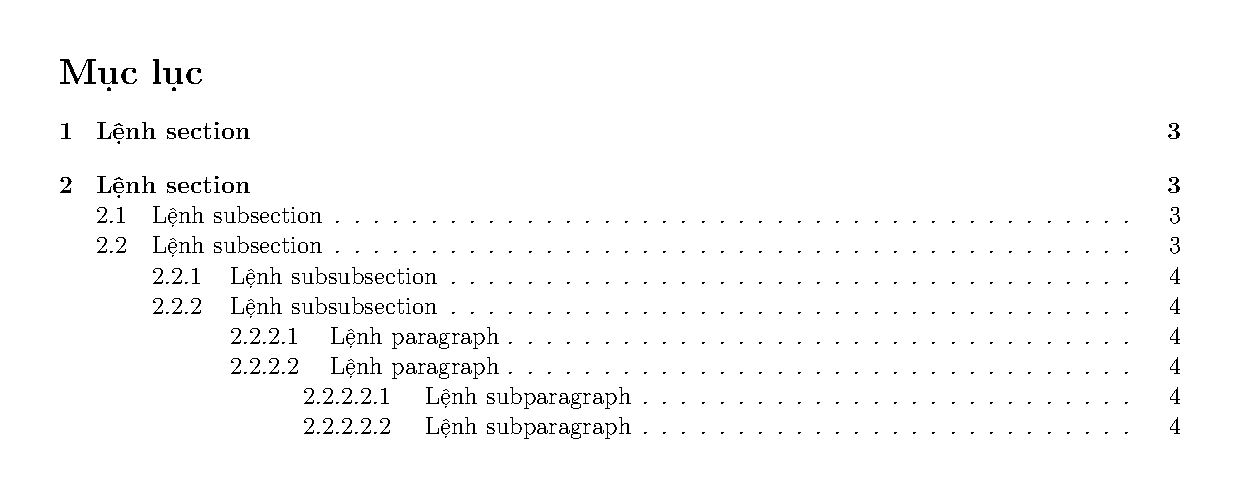
\includegraphics[scale=.8]{section-subparagraph-article}
				}
				\vspace*{-1cm}
				\subfloat[Mục lục trong lớp report]{
					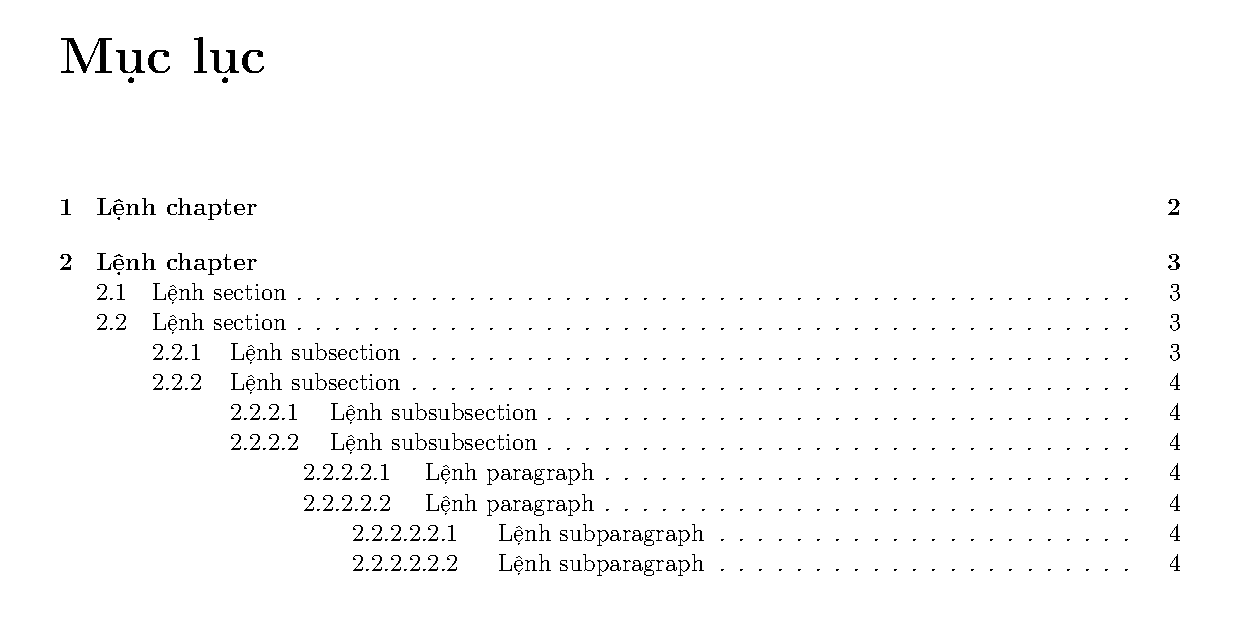
\includegraphics[scale=.8]{chapter-subparagraph-report}
				}
				\vspace*{-1cm}
				\subfloat[Mục lục trong lớp book]{
					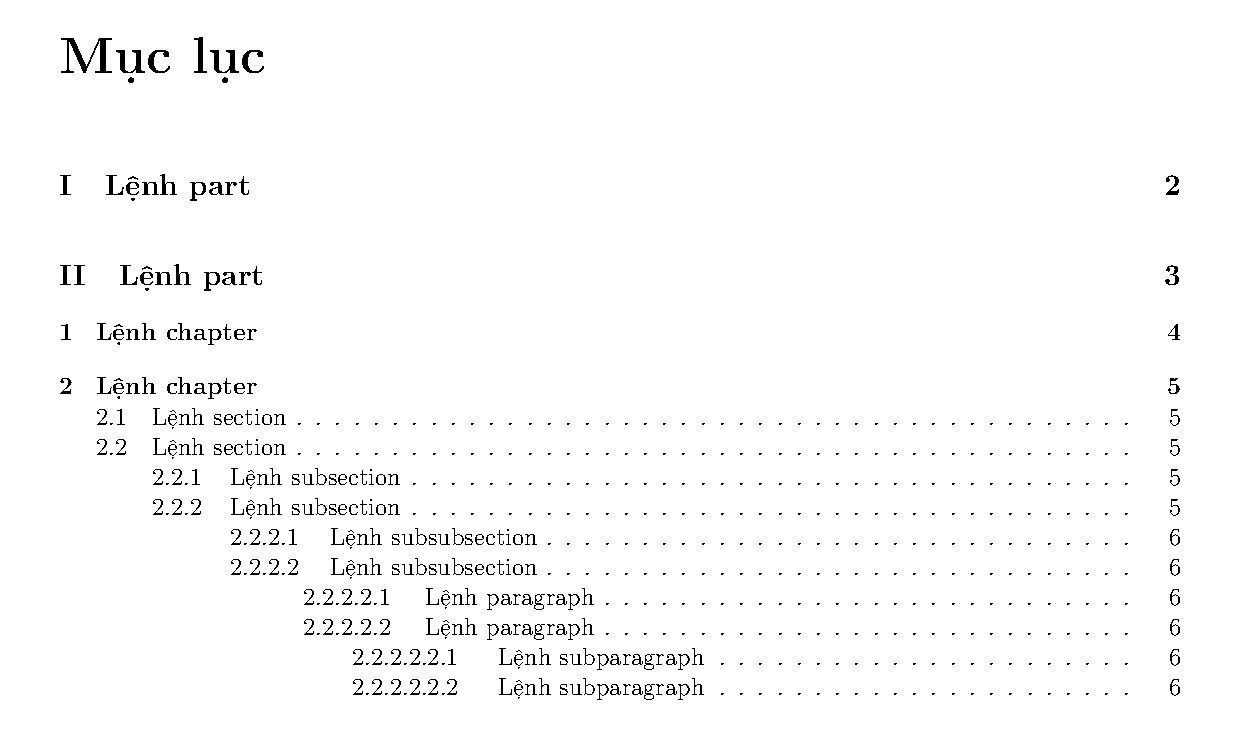
\includegraphics[scale=.8]{part-subparagraph-book}
				}				
				\caption{Mô tả về cách đánh số trong mục lục ứng với các lớp tài liệu của \LaTeX} \label{Ex:danhso-mucluc}
			\end{figure}
\newpage
		\item \ex{\ref{Ex:danhso-noidung}} Mô tả về hình thức trình bày khi cho hiện số của những cấp độ bị ẩn trong lớp \Verb|article| (tương tự cho các lớp \Verb|report| và \Verb|book|).
			\begin{figure}[h]
				\begin{center}
					\vspace*{-1cm}
					\subfloat[Code \LaTeX]{
						\hspace*{-1cm}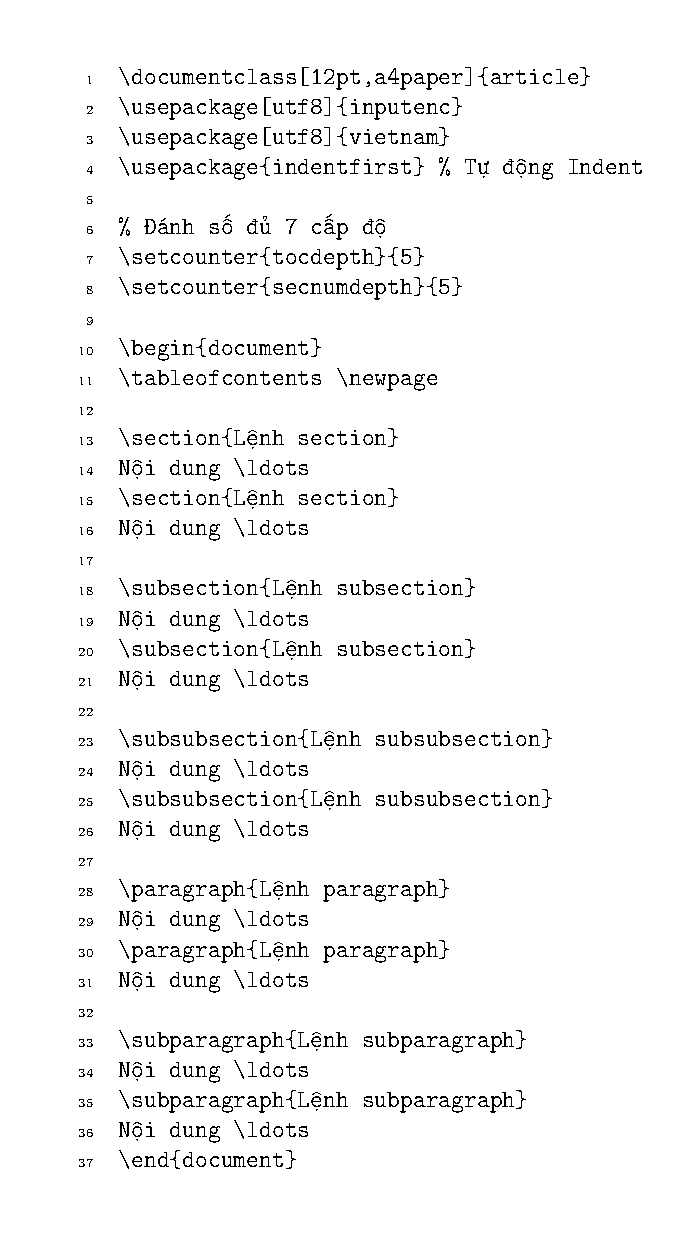
\includegraphics[scale=.8]{section-subparagraph-article-1}
					}
					\subfloat[Kết quả phần nội dung]{
						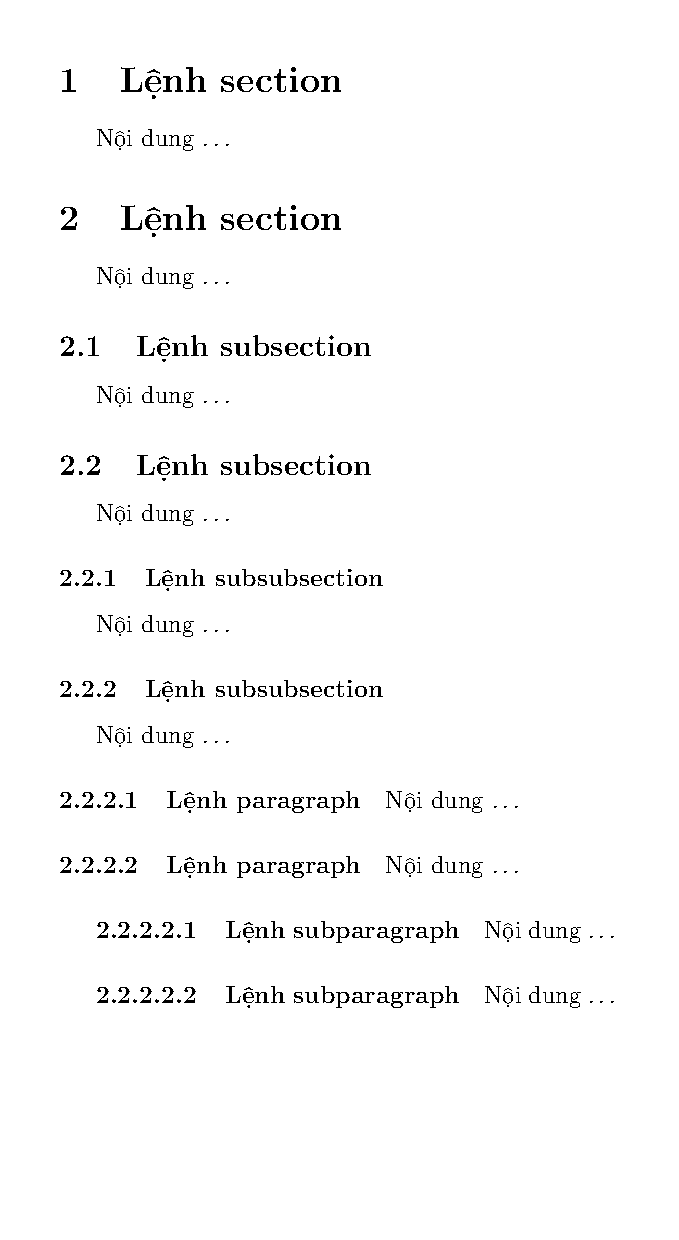
\includegraphics[scale=.8]{section-subparagraph-article-2}
					}
				\end{center}
				\caption{Mô tả các đánh số và hình thức trình bày của các đề mục trong lớp article}\label{Ex:danhso-noidung}
			\end{figure}
	\end{itemize}

\subsection{Định nghĩa lại các lệnh paragraph và subparagraph}
	\begin{itemize}
		\item Trên \ex{\ref{Ex:danhso-noidung}}, nội dung của lệnh \Verb|\paragraph| và \Verb|\subparagraph| không tự động xuống dòng mới và lệnh \Verb|\subparagraph| cũng không tự động canh thẳng hàng như các mục trên nó.
		
		\item Để làm cho các lệnh \Verb|\paragraph| và \Verb|\subparagraph| có định dạng tương tự như các mục trên nó, chúng ta định nghĩa lại chúng như bên dưới. Kết quả được mô tả trên \ex{\ref{Ex:danhso-noidung-2}}.
			\begin{itemize}
				\item Định nghĩa các lệnh \Verb|\parasection| và \Verb|\subparasection| từ các lệnh \Verb|\paragraph| và \Verb|\subparagraph| để chúng có định dạng tương tự như các mục trên nó:
\begin{Verbatim}[xleftmargin=10mm, numbers=left]
\newcommand{\parasection}[1]{
	\paragraph{#1}\mbox{}\medskip\par}

\newcommand{\subparasection}[1]{{\setlength{\parindent}{0pt}
	\subparagraph{#1}\mbox{}\medskip\par}}
\end{Verbatim}

				\item Nếu không muốn nội dung tự động thụt vào đầu dòng như \ex{\ref{Ex:danhso-noidung}}, thì không khai báo \Verb|\usepackage{indentfirst}| và thay lệnh \Verb|\par| thành lệnh \Verb|\\|.

				\begin{figure}[h]
					\begin{center}
						\vspace{-1cm}
						\subfloat[Code \LaTeX]{
							\hspace*{-1cm}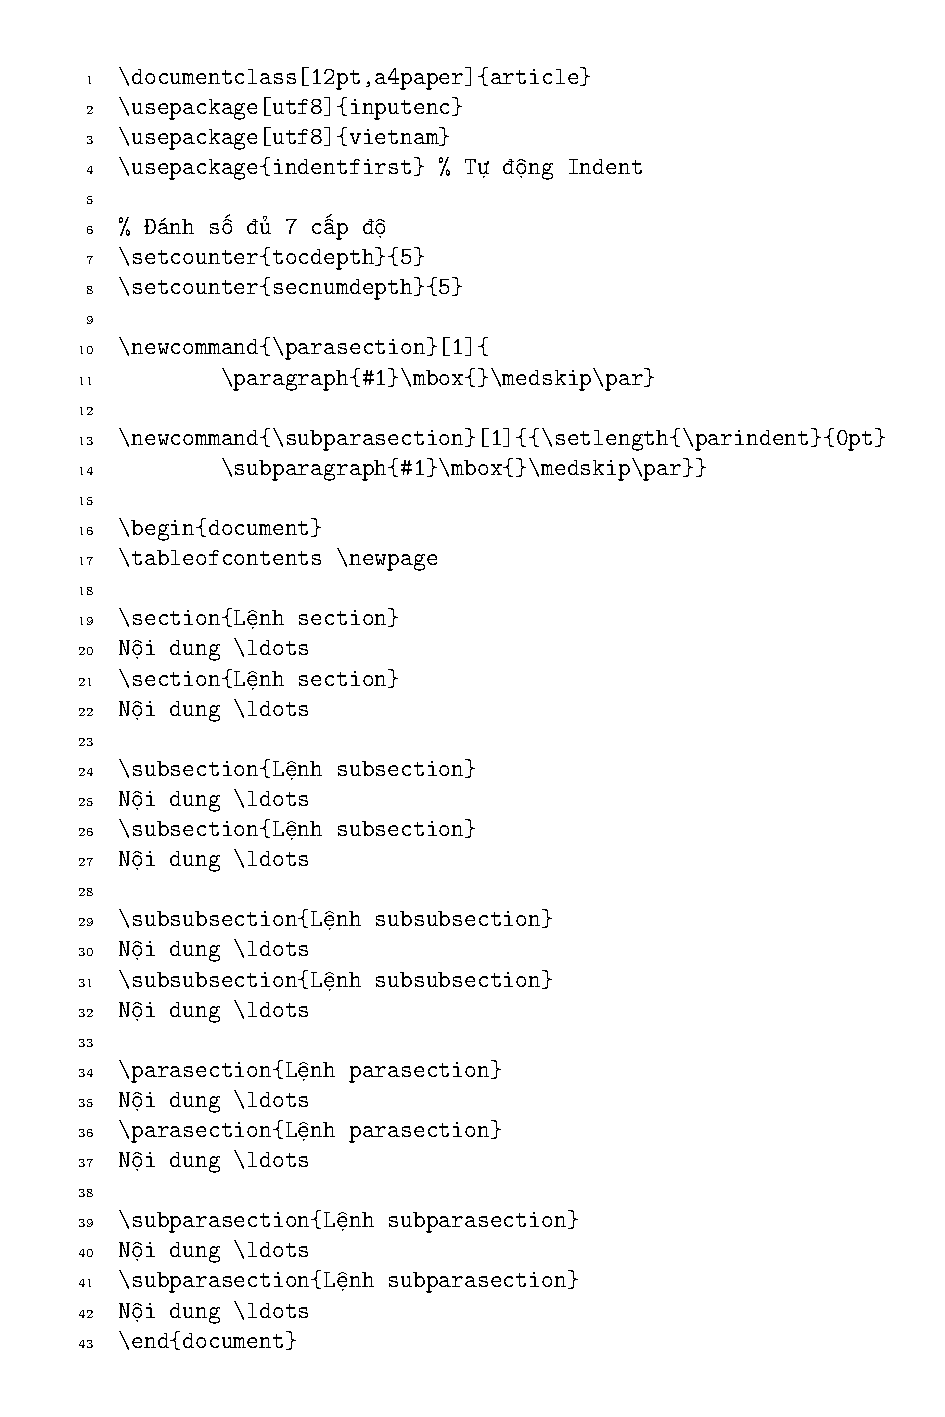
\includegraphics[scale=.8]{section-subparagraph-article-3}
						}\hspace*{-1.5cm}
						\subfloat[Kết quả phần nội dung]{
							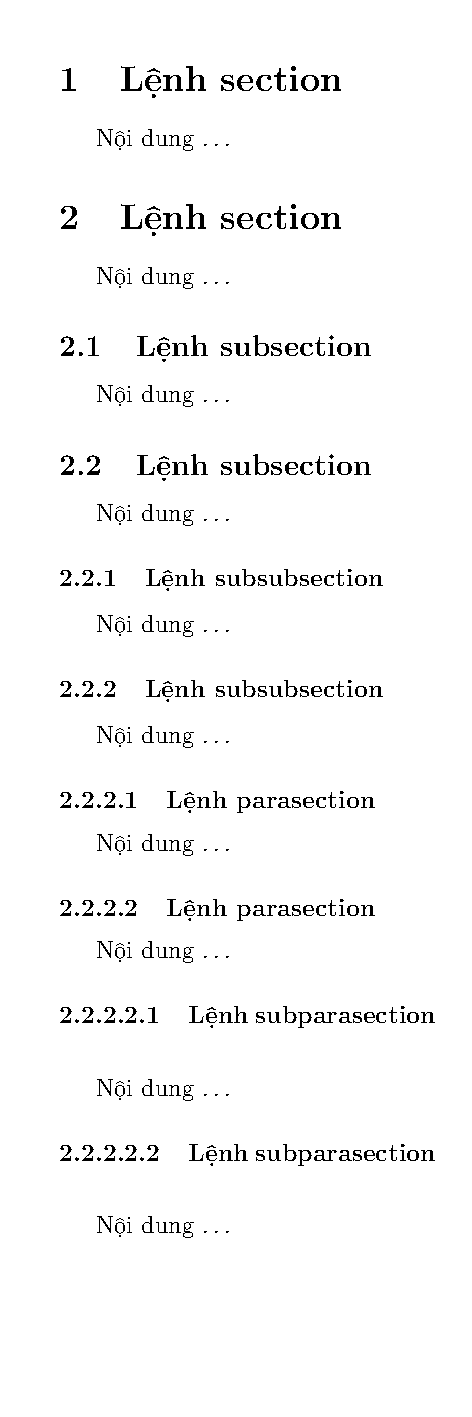
\includegraphics[scale=.8]{section-subparagraph-article-4}
						}
					\end{center}
					\caption{Mô tả các đánh số và hình thức trình bày của các đề mục trong lớp article}\label{Ex:danhso-noidung-2}
					\vspace{-1cm}
				\end{figure}
			\end{itemize}
	\end{itemize}

\section{Thay đổi cách đánh số mặc định của các cấp độ trong các lớp của \LaTeX}
	\begin{itemize}
		\item Theo mặc định, các lớp \Verb|article|, \Verb|report| và \Verb|book| sẽ đánh số mặc định như trong mô tả ở \ex{\ref{Ex:danhso-mucluc}}.
		
		\item Các biến đếm cho các phần, các chương và các mục ứng với \Verb|article|, \Verb|report| và \Verb|book| trong trong tài liệu \LaTeX\ được cho trên \tab{\ref{Tab:biendem-cautruc}}:
			\begin{table}[h]
				\begin{center}
					\begin{tabular}{llll}\toprule
					\multicolumn{2}{c}{\head{Biến đếm và lệnh tương ứng}} & \multicolumn{2}{c}{\head{Nhãn dùng hiển thị}} \\ \midrule
					\head{CounterName} & \head{Lệnh} & \head{Label} & \head{Mô tả} \\ \midrule
					\Verb|part| & \Verb|\thepart| & \Verb|\Roman| & I, II, III,\ldots\\ \midrule
					\Verb|chapter| & \Verb|\thechapter| & \Verb|\roman| & i, ii, iii,\ldots\\ \midrule
					\Verb|section| & \Verb|\thesection| & \Verb|\Alph| & A, B, C,\ldots \\ \midrule
					\Verb|subsection| & \Verb|\thesubsection| & \Verb|\alph| & a, b, c, \ldots \\ \midrule
					\Verb|subsubsection| & \Verb|\thesubsubsection| & \Verb|\arabic| & 1, 2, 3,\ldots \\ \midrule
					\Verb|paragraph| & \Verb|\thesubsection| & \Verb|\fnsymbol| & \\ \midrule
					\Verb|subparagraph| & \Verb|\thesubparagraph| &  & \\ \bottomrule
					\end{tabular}
				\end{center}
				\caption{Các biến đếm cho các phần, các chương và các mục trong tài liệu \LaTeX} \label{Tab:biendem-cautruc}
			\end{table}
		
		\item Thay đổi cách đánh số mặc định cho các mục của các lớp \Verb|article|, \Verb|report| và \Verb|book| với cú pháp như sau (chúng ta có thể kết hợp các \Verb|Label| với nhau): với \Verb|CounterName| và \Verb|Label| được cho trên \tab{\ref{Tab:biendem-cautruc}}.
			\begin{verbatim}
				\renewcommand\theCounterName{\Label{CounterName}}
			\end{verbatim}			
		
		\item \ex{\ref{Ex:thaydoi-label-article}} mô tả về thay đổi cách đánh số ứng với các mục trong lớp \Verb|article| như mô tả trên \tab{\ref{Tab:label-cautruc}}.				
		
		\begin{table}[h]
				\begin{center}
					\begin{footnotesize}
						\begin{tabular}{llcl}\toprule
							\head{Lớp} & \head{Cấp độ} & \head{Hiển thị} & \head{Lệnh}  \\ \midrule
							\multirow{7}{*}{\command{article}} & \Verb|section| & \textbf{A} & \Verb|\renewcommand\thesection{\Alph{section}}|  \\ \cmidrule{2-4}
							& \Verb|subsection| & \textbf{I} & \Verb|\renewcommand\thesubsection{\Roman{subsection}}| \\ \cmidrule{2-4}
							& \Verb|subsubsection| & \textbf{1} & \Verb|\renewcommand\thesubsubsection{\arabic{subsubsection}}| \\ \cmidrule{2-4}
							& \Verb|paragraph| & \textbf{a} & \Verb|\renewcommand\theparagraph{\alph{paragraph}}| \\ \cmidrule{2-4}
							& \Verb|subparagraph| & \textbf{i} & \Verb|\renewcommand\thesubparagraph{\roman{subparagraph}}| \\ \bottomrule
						\end{tabular}
					\end{footnotesize}
				\end{center}
				\caption{Ví dụ thay đổi cách đánh số mặc định cho lớp article} \label{Tab:label-cautruc}
			\end{table}
			
			\begin{figure}
				\begin{center}
					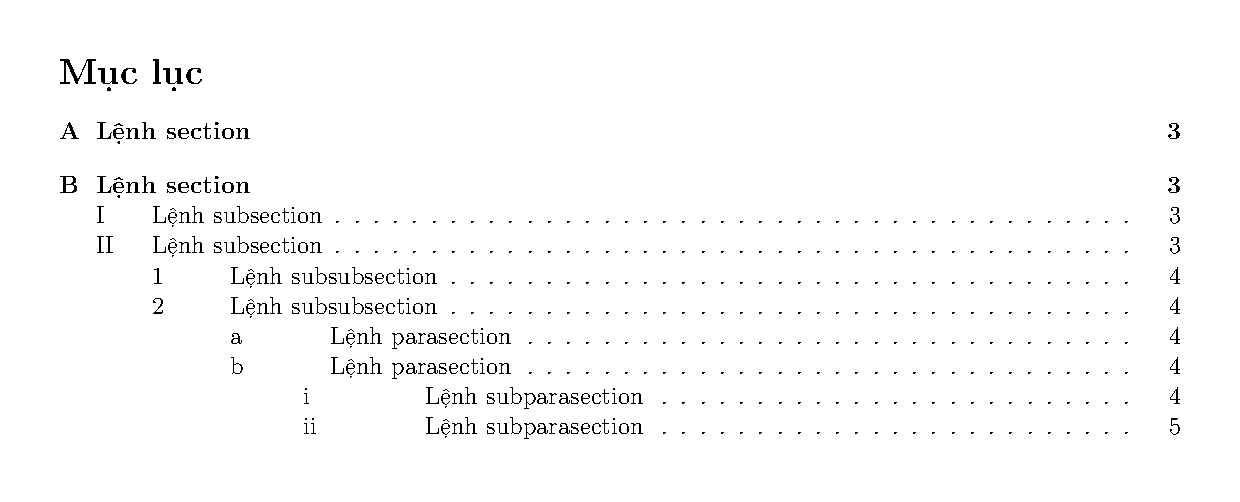
\includegraphics[scale=.75]{section-subparagraph-article-5}
				\end{center}
				\caption{Mô tả về thay đổi cách đánh số ứng với lớp article} \label{Ex:thaydoi-label-article}
			\end{figure}
\newpage			
		\item Thực hiện tương tự cho các lớp \Verb|report| và \Verb|book|.
	\end{itemize}
\end{document}
